\documentclass[11pt,a4paper]{report}
\usepackage[utf8]{inputenc}
\usepackage[T1]{fontenc}
\usepackage[english, italian, croatian]{babel}
\usepackage{amsmath, amsfonts, amssymb}
\usepackage{graphicx}
\usepackage{fancyhdr}
\usepackage{color}
\usepackage {tikz}
\usepackage{pgfplots}
\usetikzlibrary {positioning}
\usepackage{tocloft}
\usepackage[hidelinks, unicode]{hyperref}
\usepackage[section]{placeins}
\usepackage[final]{pdfpages}
\bibliographystyle{ieeetr}%ieeetr, abbrv
\pgfplotsset{compat=1.15}
\usepackage{listings}
\usepackage{appendix}
%\usepackage{chngcntr}	%Continuous footnote numbering
%\counterwithout{footnote}{chapter} %Continuous footnote numbering
\tolerance=1
\emergencystretch=\maxdimen %poravnavanje
\hyphenpenalty=10000 % no hyphenation
\hbadness=10000	
%\usepackage{helvet}
%\renewcommand{\familydefault}{\sfdefault} % promjeni font
%\renewcommand{\rmdefault}{phv}
\renewcommand{\cftsecleader}{\cftdotfill{\cftdotsep}}
\addto{\captionscroatian}{\renewcommand{\bibname}{Literatura}}
\setcounter{chapter}{-1} % zero-based numbering
\pagenumbering{Roman}

\newcommand{\kolegij}{Diplomski rad}
\newcommand{\naslovRada}{Automatiziranje testiranja web aplikacija koristeći javascript frameworkove Playwright i Cypress \\ {\large Diplomski rad}} 
\newcommand{\mailFriendlynaslovRada}{Master's Thesis - JS Testing Frameworks}

\author{
Kristijan Cetina \\{\small JMBAG: 2424011721} \\ {\href{mailto:kristijan.cetina@icloud.com?subject=\mailFriendlynaslovRada}{{\footnotesize kcetina@student.unipu.hr}}}} 
\title{\naslovRada}
\date{Pula, \today}

\begin{document}
\pgfplotsset{width=\textwidth,compat=newest}

%\begin{titlepage}
%\clearpage
%\begin{center}
%\begin{Large}
%ISTARSKO VELEUČILIŠTE\\
%UNIVERSIT\`{A} ISTRIANA DI SCIENZE APPLICATE\\
%Stručni studij politehnike\end{Large}
%\end{center}
%\vspace{3cm}
%{\let\newpage\relax\maketitle}
%\thispagestyle{empty}
%
%\end{titlepage}

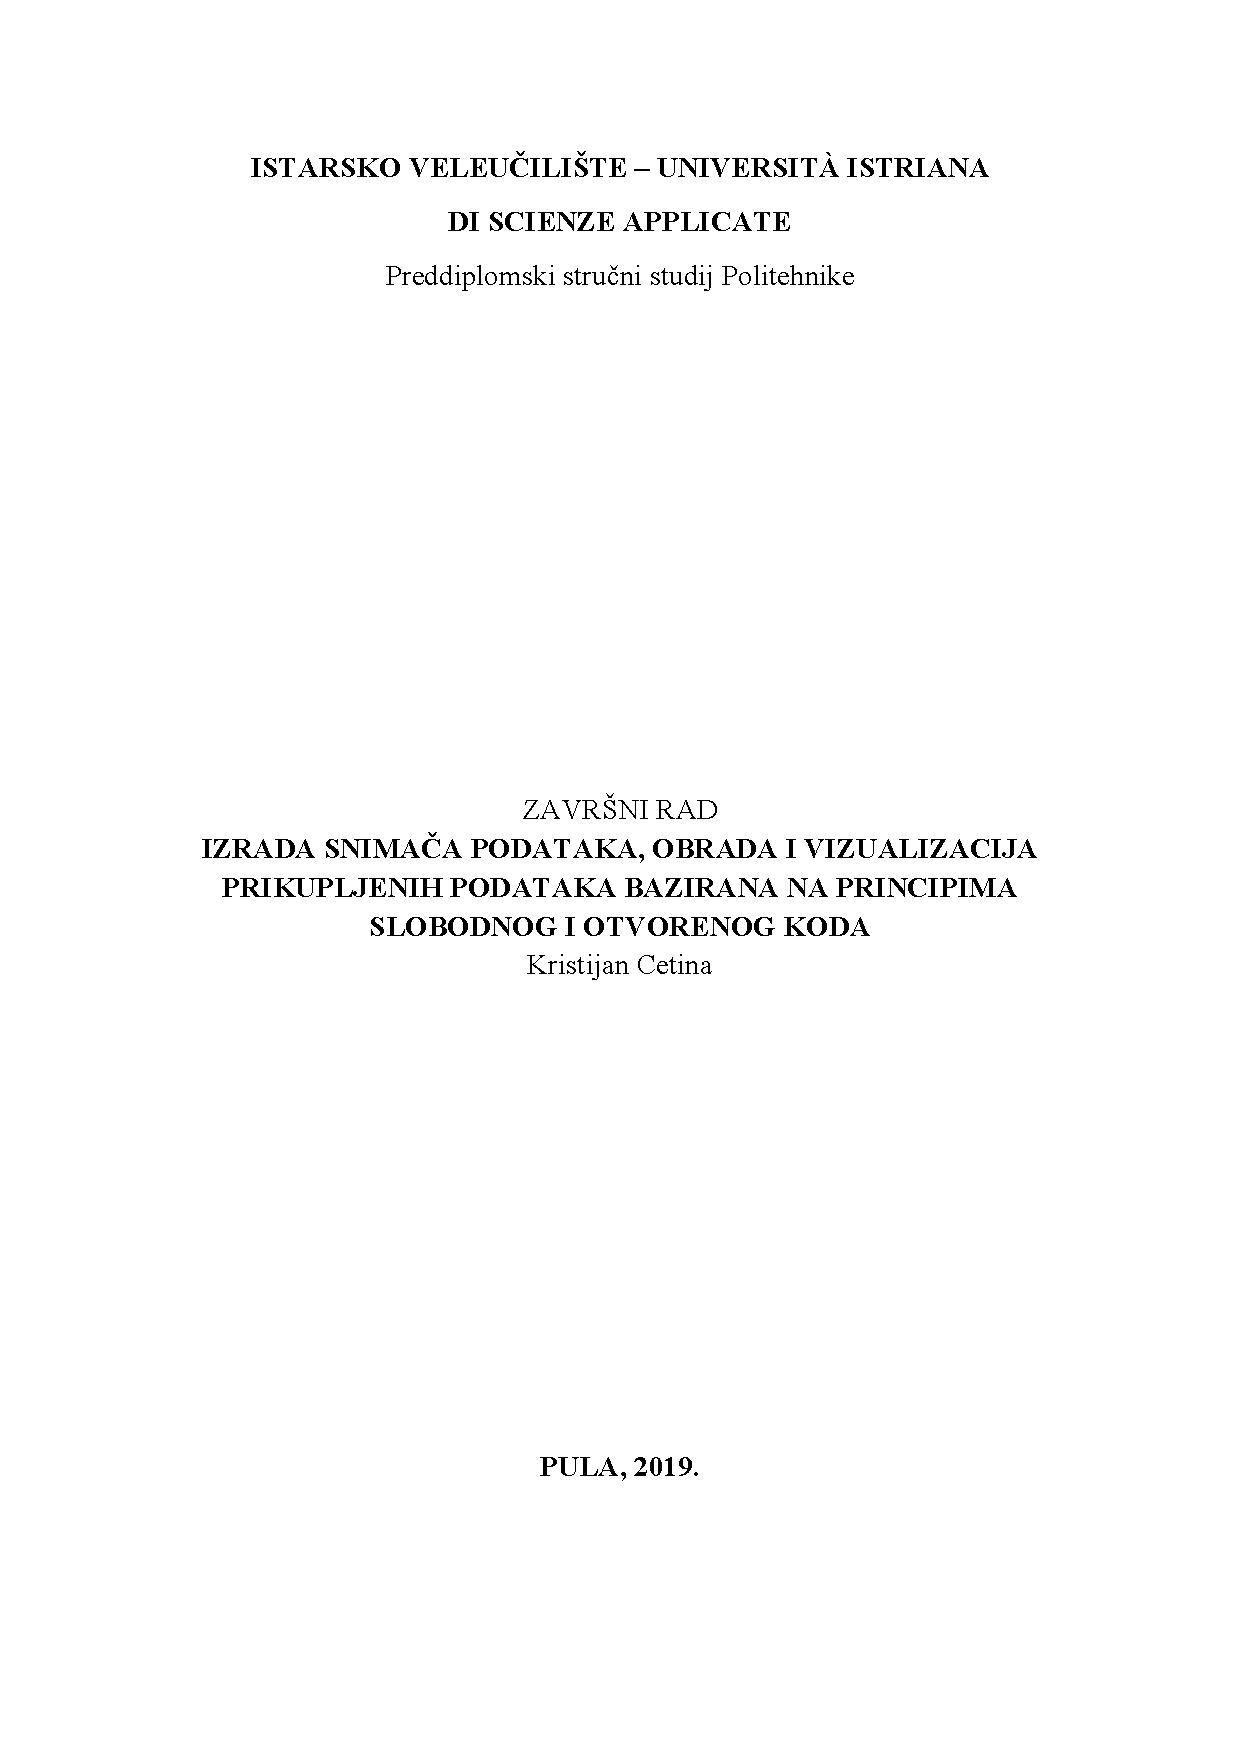
\includepdf[pages={1-},fitpaper]{pocetne_stranice.pdf}
\setcounter{page}{1}
\chapter*{Zahvala}
Zahvaljujem svojem mentoru  na izdvojenom vremenu i podršci, kako na izradi ovog rada, tako i tijekom cijelog studiranja na Fakultetu informatike.

Zahvaljujem se i svojim timskim kolegama, s kojima sam od samog početka sudjelovao na svim timskim zadatcima i njihovoj pomoći pri individualnom radu. Bez vas ovo iskustvu ne bi bilo niti upola zabavno kao što je bilo.

Zahvaljujem se i svim ostalim profesorima i djelatnicima  na nesebičnoj potpori kada je god to bilo potrebno.

Naposljetku veliko hvala mojoj obitelji na potpori i razumijevanju tijekom mojeg ponovnog studiranja.

\chapter*{Izjava o samostalnosti izrade završnog rada}
Izjavljujem da sam završni rad na temu \textbf{\emph{\naslovRada}} samostalno izradio uz pomoć mentora,  koristeći navedenu stručnu literaturu i znanje stečeno tijekom studiranja.
Završni rad pisan je u duhu hrvatskoga jezika.
\vspace{\fill}
\begin{flushright}
Student: Kristijan Cetina\\
\vspace{15mm}
--------------------------------------------------------------
\end{flushright}
\section*{Sažetak}\label{sazetak_hr}
\addcontentsline{toc}{chapter}{\nameref{sazetak_hr}}
Često se kaže da je testiranje softvera jednako važno kao i samo kodiranje. 
Kako se kompleksnost aplikacija povećava, tako raste i vjerojatnost pojave pogrešaka koje mogu negativno utjecati na korisničko iskustvo. 
Da bismo to spriječili, koristimo razne tehnike testiranja, a jedna od njih je testiranje klijentskih komponenti.

Ovaj rad se fokusira na korištenje Microsoftovog alata Playwright za testiranje klijentskih komponenti. 
Playwright je popularan izbor za end-to-end testiranje modernih web aplikacija jer omogućuje pouzdano testiranje na različitim preglednicima i platformama. 
Njegove glavne prednosti uključuju podršku za najnovije web tehnologije, jednostavnu sintaksu i mogućnost pisanja robusnih i održavanih testova.

\subsection*{Ključne riječi}\label{kw_hr}
\addcontentsline{toc}{section}{\nameref{kw_hr}}
\textit{Playwright, JavaScript, open-source}

\section*{Sommario}\label{sazetak_it}
\addcontentsline{toc}{chapter}{\nameref{sazetak_it}}
Si dice spesso che testare il software sia importante quanto la codifica stessa.
Con l'aumento della complessità delle applicazioni, aumenta anche la probabilità di errori che possono influire negativamente sull'esperienza utente.
Per prevenirlo, utilizziamo diverse tecniche di test, una delle quali è il test dei componenti client-side.

Questo documento si concentra sull'utilizzo di Playwright di Microsoft per testare i componenti client-side.
Playwright è una scelta popolare per i test end-to-end delle moderne applicazioni web in quanto consente test affidabili su diversi browser e piattaforme.
I suoi principali vantaggi includono il supporto per le ultime tecnologie web, una sintassi semplice e la capacità di scrivere test robusti e manutenibili.

\subsection*{Parole chiave:}\label{kw_it}
\addcontentsline{toc}{section}{\nameref{kw_it}}
\textit{Playwright, JavaScript, open-source}

\section*{Abstract}\label{sazetak_en}
\addcontentsline{toc}{chapter}{\nameref{sazetak_en}}
It's often said that testing software is equally important as coding itself.

 As application complexity grows, so does the likelihood of errors that can negatively impact the user experience.
 To prevent this, we use various testing techniques, one of which is testing client-side components.

This paper focuses on using Microsoft's Playwright for testing client-side components.
Playwright is a popular choice for end-to-end testing of modern web applications as it enables reliable testing across different browsers and platforms.
Its main advantages include support for the latest web technologies, simple syntax, and the ability to write robust and maintainable tests.

\subsection*{Keywords:}\label{kw_en}
\addcontentsline{toc}{section}{\nameref{kw_en}}
\textit{Playwright, JavaScript, open-source}
\chapter*{Popis oznaka i kratica}\label{TOA}
\addcontentsline{toc}{chapter}{\nameref{TOA}}

\begin{tabbing}\label{Oznake}
\hspace{60pt}\=\hspace{160pt}\=\kill
 \textbf{Oznaka} \>  \textbf{Opis} \> \textbf{Jedinica} \\ 
 t \>  vrijeme (sekunda) \> $s$ \\ 
 $\theta$ \>  temperatura (Celzijev stupanj) \> $^ \circ C$ \\ 
 $\nu$ \>  brzina \> $m/s$ \\ 
 s \>  udaljenost u metrima \> $m$ \\ 
 f \>  frekvencija \> $Hz$ \\ 
 C \>  kapacitet kondenzatora \> $F$ \\ 
  \> Veličina memorije \> MB, 1MB = 1048576 bajtova
\end{tabbing}


\begin{tabbing}
\hspace{80pt}\=\kill
\textbf{Kratica} \> \textbf{Opis} \\ 
 GPS \> Global Positioning System - Sustav globalnog pozicioniranja  \\ 
 SD \> Secure Digital - format memorijske kartice\\ 
 $\mu$SD, microSD \> mikro Secure Digital - kartica manjih fizičkih dimenzija \\ 
 PWM \> Pulse Width Modulation - Pulsno-širinska modulacija \\ 
 IDE \> Integrated Development Environment  - Integrirano razvojno okruženje \\ 
 GND \> Točka nultog potencijala \\ 
 SW \> Software \\ 
 HW \> Hardware \\ 
 NMEA \> National Marine Electronics Association \\ 
 UTC \> Coordinated Universal Time - Standardno vrijeme \\ 
 .csv \> comma-separated values - vrijednosti odvojene zarezom \\ 
 .md \> Markdown datoteka
\end{tabbing} 

\tableofcontents
%\listoftables	%ako ih ima puno prebaci na kraj dokumenta
\newpage

\pagenumbering{arabic}
\chapter{Uvod i opis zadatka}\label{OpisIOgranicenja}
U dinamičnom svijetu razvoja softvera, automatizacija testiranja igra ključnu ulogu u osiguravanju kvalitete proizvoda.
End-to-end (E2E) testiranje je pristup koji omogućuje simulaciju stvarnog korisničkog iskustva kroz cijeli sustav, od početka do kraja.
Cilj ovih testova je potvrditi da svi dijelovi sustava funkcioniraju zajedno na predviđeni način.
Sa sve većom složenošću softverskih sustava i potrebom za bržim izdanjima, automatsko E2E testiranje postaje sve relevantnije. 
Međutim, ovo testiranje donosi sa sobom niz izazova koje je potrebno adresirati kako bi bilo učinkovito i korisno.


\section*{Opis i definicija problema}
Automatsko end-to-end testiranje softvera obuhvaća proces kreiranja, izvršavanja i održavanja testova koji provjeravaju funkcionalnost aplikacije kao cjeline.
Problem koji se istražuje u ovom radu može se definirati kroz sljedeće ključne aspekte:

Složenost Kreiranja Testova: Kreiranje automatskih E2E testova zahtijeva duboko razumijevanje svih dijelova sustava i njihovih međusobnih interakcija.
Ovo može biti izuzetno složeno u velikim i distribuiranim sustavima.

Održavanje Testova: S obzirom na česte promjene u kodu i sistemskim zahtjevima, automatski E2E testovi zahtijevaju redovno održavanje kako bi ostali relevantni.
Svaka promjena može potencijalno zahtijevati modifikaciju ili kreiranje novih testova.

Izvršavanje Testova: Automatski E2E testovi često traju duže od drugih vrsta testova (kao što su unit testovi ili integracijski testovi) zbog svoje prirode koja obuhvaća cijeli sustav. 
Ovo može rezultirati dugim vremenom izvršavanja i problemima s performansama.

Pouzdanost Testova: Testovi moraju biti pouzdani, tj. rezultati testiranja moraju biti točni i konzistentni. 
Lažno pozitivni ili negativni rezultati mogu dovesti do gubitka povjerenja u testove i dodatnih troškova.

Integracija sa CI/CD Procesima: Automatsko E2E testiranje mora biti integrirano s kontinuiranim integracijskim i kontinuiranim isporučnim (CI/CD) procesima kako bi podržalo agilne prakse razvoja softvera. Ovo zahtijeva visok nivo automatizacije i orkestracije.


\section*{Struktura rada}
Struktura ovoga rada podjeljena je u logičke cjeline.
Nakon uvoda i objašnjavanja rada, u poglavlju \ref{uvodQA} - \nameref{uvodQA} objašnjen je proces testiranje i osiguranja kvalitete programskog rješenja.

Poglavlje \ref{ch_playwright} - \nameref{ch_playwright} detaljnije objašnjava korištenu biblioteku kao i njezino korištenje.

Poglavlje \ref{postdeploy} - \nameref{postdeploy} objašnjava proces testiranja nakon objave nove verzije kao i problem koji se pokušava rješiti ovim radom.

Poglavlje \ref{ch:implementacija} - \nameref{ch:implementacija} pruža detaljniji uvid u samo rješenje koje je implementirano unutar kompanije u kojoj autor trenutno radi.

Kompletan Git repozitorij ovog rada javno je dostupan na \url{https://github.com/KristijanCetina/jsTesting}

\chapter{Zaključak}\label{ch:Zakljucak}
U ovom radu prikazan je postupak izrade 


\nocite{*}
\addcontentsline{toc}{chapter}{Literatura}
\bibliography{literatura}
\listoffigures
\addcontentsline{toc}{chapter}{Popis slika}

\newpage

ovo je test
\appendix
\begin{appendices}\appendix
\chapter{Programski kod na Arduino mikroračunalu}\label{ArduinoSource}
\end{appendices}

\end{document}